%%%%%%%%%%%%%%%%%%%%%%%%%%%%%%%%%%%%%%%%%
% Beamer Presentation
% LaTeX Template
% Version 1.0 (10/11/12)
%
% This template has been downloaded from:
% http://www.LaTeXTemplates.com
%
% License:
% CC BY-NC-SA 3.0 (http://creativecommons.org/licenses/by-nc-sa/3.0/)
%
%%%%%%%%%%%%%%%%%%%%%%%%%%%%%%%%%%%%%%%%%

%----------------------------------------------------------------------------------------
%	PACKAGES AND THEMES
%----------------------------------------------------------------------------------------

\documentclass{beamer}

\mode<presentation> {

% The Beamer class comes with a number of default slide themes
% which change the colors and layouts of slides. Below this is a list
% of all the themes, uncomment each in turn to see what they look like.

%\usetheme{default}
%\usetheme{AnnArbor}
%\usetheme{Antibes}
%\usetheme{Bergen}
%\usetheme{Berkeley}
%\usetheme{Berlin}
%\usetheme{Boadilla}
%\usetheme{CambridgeUS}
%\usetheme{Copenhagen}
\usetheme{Darmstadt}
%\usetheme{Dresden}
%\usetheme{Frankfurt}
%\usetheme{Goettingen}
%\usetheme{Hannover}
%\usetheme{Ilmenau}
%\usetheme{JuanLesPins}
%\usetheme{Luebeck}
%\usetheme{Madrid}
%*\usetheme{Malmoe}
%\usetheme{Marburg}
%\usetheme{Montpellier}
%\usetheme{PaloAlto}
%\usetheme{Pittsburgh}
%\usetheme{Rochester}
%\usetheme{Singapore}
%\usetheme{Szeged}
%\usetheme{Warsaw}

% As well as themes, the Beamer class has a number of color themes
% for any slide theme. Uncomment each of these in turn to see how it
% changes the colors of your current slide theme.

%\usecolortheme{albatross}
%\usecolortheme{beaver}
%\usecolortheme{beetle}
%\usecolortheme{crane}
%\usecolortheme{dolphin}
%\usecolortheme{dove}
%\usecolortheme{fly}
%\usecolortheme{lily}
\usecolortheme{orchid}
%\usecolortheme{rose}
%\usecolortheme{seagull}
%\usecolortheme{seahorse}
%\usecolortheme{whale}
%\usecolortheme{wolverine}

%\setbeamertemplate{footline} % To remove the footer line in all slides uncomment this line
%\setbeamertemplate{footline}[page number] % To replace the footer line in all slides with a simple slide count uncomment this line

%\setbeamertemplate{navigation symbols}{} % To remove the navigation symbols from the bottom of all slides uncomment this line
}


\usepackage{graphicx} % Allows including images
\usepackage{booktabs} % Allows the use of \toprule, \midrule and \bottomrule in tables
\usepackage{xspace}
\usepackage{caption}
\usepackage{subfigure}
\usepackage[english,brazil]{babel}
\usepackage[utf8]{inputenc}

%Renomeia o nome padrao das figuras.
\renewcommand{\figurename}{Figura}
\renewcommand{\tablename}{Tabela}
%----------------------------------------------------------------------------------------
%	TITLE PAGE
%----------------------------------------------------------------------------------------

\title[Computação Gráfica]{Métodos de Rendering de Superfície} % The short title appears at the bottom of every slide, the full title is only on the title page

\author{Uéliton Freitas} % Your name
\institute[UFMS] % Your institution as it will appear on the bottom of every slide, may be shorthand to save space
{
Universidade Católica Dom Bosco - UCDB \\ % Your institution for the title page
\medskip
\textit{freitas.ueliton@gmail.com} % Your email address
}
\date{\today} % Date, can be changed to a custom date


\begin{document}

\begin{frame}
\titlepage % Print the title page as the first slide
\end{frame}

\begin{frame}
\frametitle{Sumário} % Table of contents slide, comment this block out to remove it
\tableofcontents % Throughout your presentation, if you choose to use \section{} and \subsection{} commands, these will automatically be printed on this slide as an overview of your presentation
\end{frame}




%----------------------------------------------------------------------------------------
%	PRESENTATION SLIDES
%----------------------------------------------------------------------------------------

%------------------------------------------------
\section{Introdução} 
%------------------------------------------------

%\section{Speeded-Up Robust Features - SURF} % A subsection can be created just before a set of slides with a common theme to further break down your presentation into chunks
%\section{Baf Of Features and Colors}

%\section{Refer\^encias}
%%%%%%%%%%%%%%%%%%%%%%%%%%%%%%%%%%%%%%%%%%%%%%%%%%%%%%%%%%%%%%%%%%%%%%%%%%%%%%%%%%%%%%%%%%
\begin{frame}
\frametitle{Introdução}

		\begin{figure}[!h]
			\begin{center}
			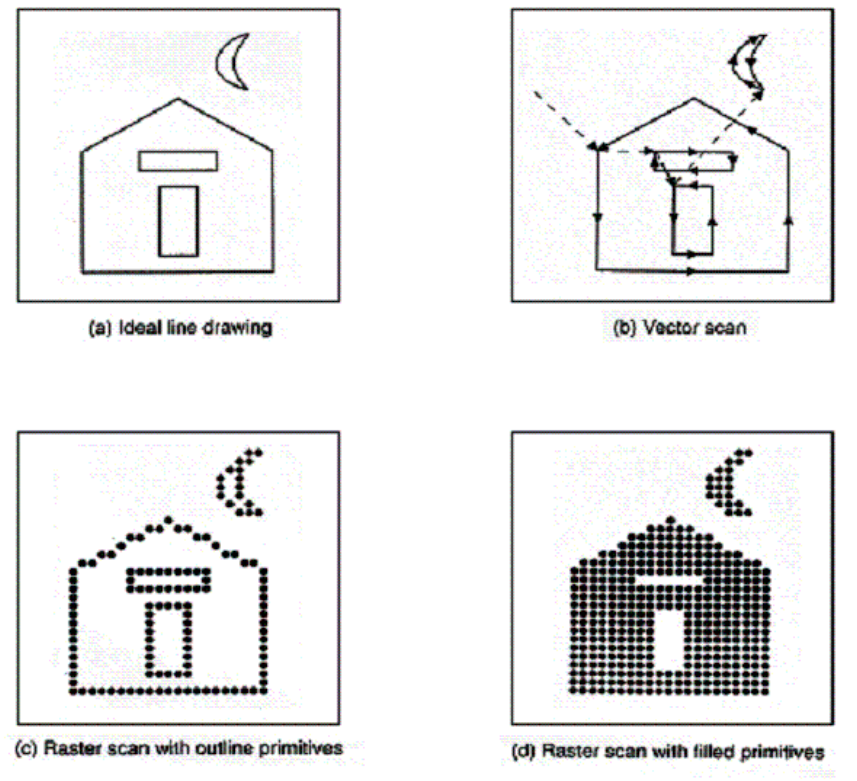
\includegraphics[width=0.6\textwidth]{Figures/IMG}
			\caption{Imagen vetorial $\times$ Imagem Matricial}
			\end{center}
		\end{figure}
	
\end{frame}



%%%%%%%%%%%%%%%%%%%%%%%%%%%%%%%%%%%%%%%%%%%%%%%%%%%%%%%%%%%%%%%%%%%%%%%%%%%%%%%%%%%%%%%%%%
\begin{frame}
\frametitle{Introdução}

		\begin{block}{Problemas}
		\begin{itemize}
			\item Traçar primitivas geométricas (segmentos de retas, polígonos, circunferências, elipses, curvas,...) no dispositivo matricial.
			\item ``rastering''= conversão vetorial $\to$ matricial.
			
			\item Como ajustar uma curva, definida como coordenadas reais em um sistema de coordenadas inteiras cujos ``pontos'' tem área associada. 						 
		\end{itemize}
	\end{block}
	
\end{frame}


%%%%%%%%%%%%%%%%%%%%%%%%%%%%%%%%%%%%%%%%%%%%%%%%%%%%%%%%%%%%%%%%%%%%%%%%%%%%%%%%%%%%%%%%%%
\begin{frame}
\frametitle{Introdução}

		\begin{block}{Problemas}
		\begin{itemize}
			\item Traçar primitivas geométricas (segmentos de retas, polígonos, circunferências, elipses, curvas,...) no dispositivo matricial.
			\item ``rastering''= conversão vetorial $\to$ matricial.
			
			\item Como ajustar uma curva, definida como coordenadas reais em um sistema de coordenadas inteiras cujos ``pontos'' tem área associada. 						 
		\end{itemize}
	\end{block}
	
\end{frame}

%%%%%%%%%%%%%%%%%%%%%%%%%%%%%%%%%%%%%%%%%%%%%%%%%%%%%%%%%%%%%%%%%%%%%%%%%%%%%%%%%%%%%%%%%%
\begin{frame}
\frametitle{Introdução}

		\begin{figure}[!h]
			\begin{center}
			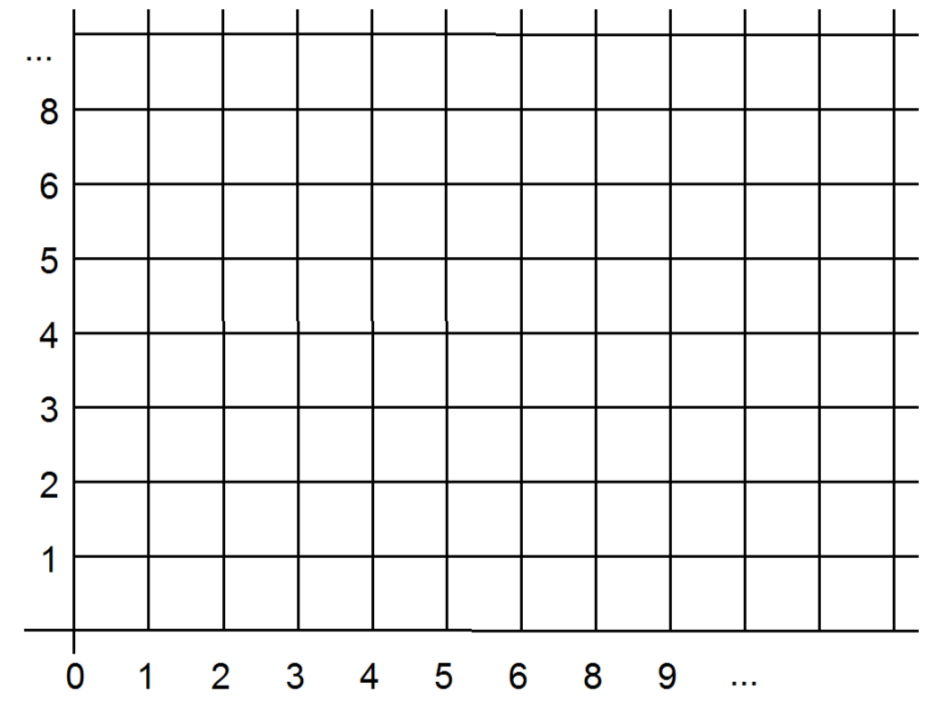
\includegraphics[width=0.6\textwidth]{Figures/DevSisCoo}
			\caption{Sistema de coordenadas de dispositivo.}
			\end{center}
		\end{figure}
	
\end{frame}


%%%%%%%%%%%%%%%%%%%%%%%%%%%%%%%%%%%%%%%%%%%%%%%%%%%%%%%%%%%%%%%%%%%%%%%%%%%%%%%%%%%%%%%%%%
\section{Conversão de Segmento de Reta}
\begin{frame}
\frametitle{Conversão de Segmento de Reta}

		\begin{block}{Conversão de Segmento de Reta}
		\begin{itemize}
			\item Dados pontos extremos em coordenadas de dispositivo
			\begin{itemize}
				\item $P_0 (x_0,y_0)$.
				\item $P_{end} (x_{end},y_{end})$.
			\end{itemize}
			\item Determinar quais pixels devem ser ``acesos'' para gerar uma boa aproximação do segmento de reta ideal.
		\end{itemize}
	\end{block}
	
\end{frame}

%%%%%%%%%%%%%%%%%%%%%%%%%%%%%%%%%%%%%%%%%%%%%%%%%%%%%%%%%%%%%%%%%%%%%%%%%%%%%%%%%%%%%%%%%%
\section{Conversão de Segmento de Reta}
\begin{frame}
\frametitle{Conversão de Segmento de Reta}

		\begin{block}{Conversão de Segmento de Reta}
		\begin{itemize}
			\item Características desejáveis:
			\begin{itemize}
				\item Linearidade.
				\item Precisão.
				\item Espessura (Densidade Uniforme).
				\item Intensidade independente de inclinação.
				\item Continuidade.
				\item Rapidez.
			\end{itemize}
		\end{itemize}
	\end{block}
	
\end{frame}

%%%%%%%%%%%%%%%%%%%%%%%%%%%%%%%%%%%%%%%%%%%%%%%%%%%%%%%%%%%%%%%%%%%%%%%%%%%%%%%%%%%%%%%%%%
\begin{frame}
\frametitle{Conversão de Segmento de Reta}

		\begin{block}{Equação da Reta}
		\begin{itemize}
			\item Usar equação explícita da reta
			\begin{equation*}
				y = m \cdot x + b
			\end{equation*}
			\item $m$ é a inclinação da reta e é dado por
			\begin{equation*}
				m = \frac{y_{end} - y_0}{x_{end} - x_0}
			\end{equation*}
			\item $b$ é a intersecção do eixo $y$ e dado por
			\begin{equation*}
				b = y_0 - m\cdot x_0
			\end{equation*}
		\end{itemize}
	\end{block}
	
\end{frame}

%%%%%%%%%%%%%%%%%%%%%%%%%%%%%%%%%%%%%%%%%%%%%%%%%%%%%%%%%%%%%%%%%%%%%%%%%%%%%%%%%%%%%%%%%%
\begin{frame}
\frametitle{Conversão de Segmento de Reta}

		\begin{block}{Algoritmos Simples}
		\begin{itemize}
			\item Varia-se $x$ unitariamente de pixel em pixel, encontrando o valor de $y$.
		\end{itemize}
	\end{block}
	
	\begin{figure}[!h]
			\begin{center}
			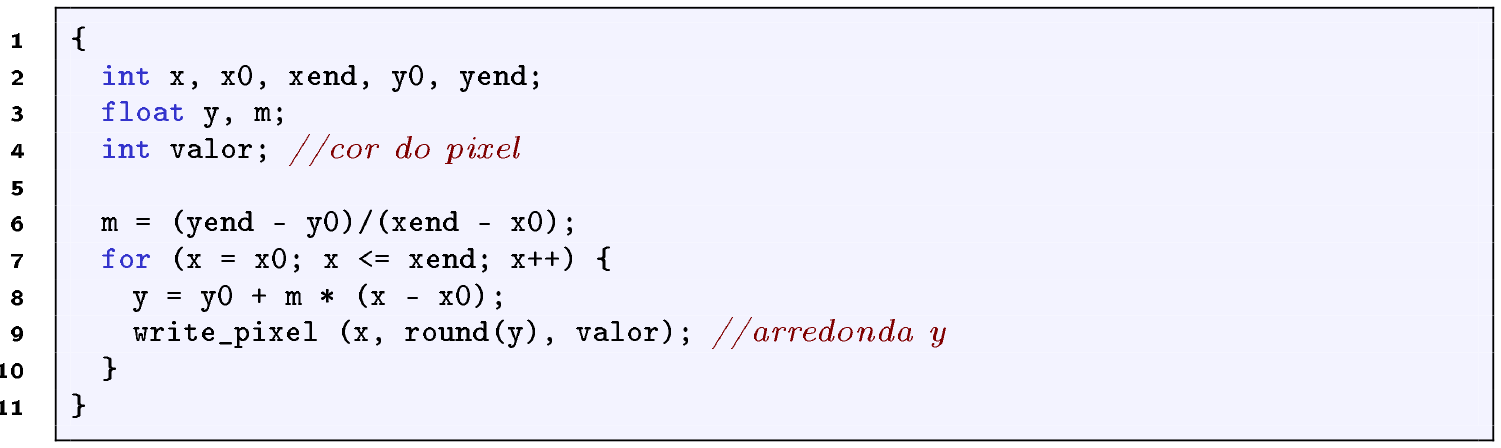
\includegraphics[width=1\textwidth]{Figures/Cod}
			\end{center}
		\end{figure}
	
\end{frame}


%%%%%%%%%%%%%%%%%%%%%%%%%%%%%%%%%%%%%%%%%%%%%%%%%%%%%%%%%%%%%%%%%%%%%%%%%%%%%%%%%%%%%%%%%%
\begin{frame}
\frametitle{Conversão de Segmento de Reta}

		\begin{block}{Algoritmos Simples}
		\begin{itemize}
			\item Na forma dada funciona apenas com segmentos em que $ 0 < m < 1$. Por que?
		\end{itemize}
	\end{block}
	
\end{frame}


%%%%%%%%%%%%%%%%%%%%%%%%%%%%%%%%%%%%%%%%%%%%%%%%%%%%%%%%%%%%%%%%%%%%%%%%%%%%%%%%%%%%%%%%%%
\begin{frame}
\frametitle{Conversão de Segmento de Reta}

		\begin{block}{Algoritmos Simples}
		\begin{itemize}
			\item Se $0 < m < 1$ a variação em $x$ é maior que em $y$. Caso não seja verdade, será traçado um segmento com buracos.
		\end{itemize}
	\end{block}
	
	\begin{figure}[!h]
			\begin{center}
			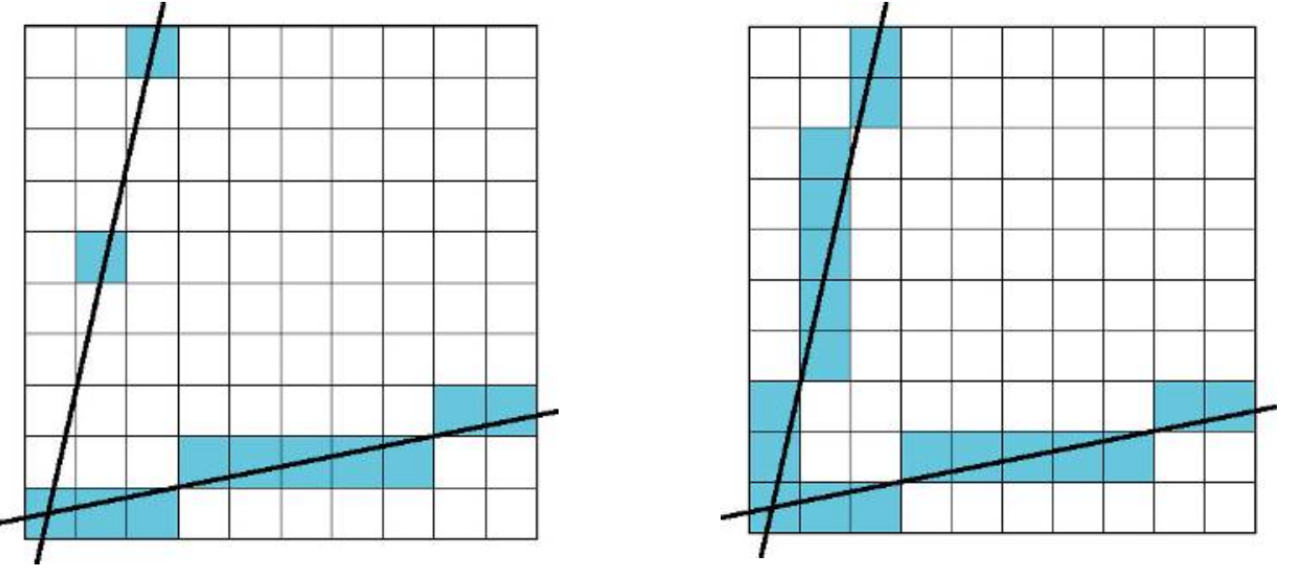
\includegraphics[width=1\textwidth]{Figures/Ret}
			\end{center}
		\end{figure}
	
\end{frame}

%%%%%%%%%%%%%%%%%%%%%%%%%%%%%%%%%%%%%%%%%%%%%%%%%%%%%%%%%%%%%%%%%%%%%%%%%%%%%%%%%%%%%%%%%%
\begin{frame}
\frametitle{Conversão de Segmento de Reta}

		\begin{block}{Algoritmos Simples}
		\begin{itemize}
			\item Se $m > 1$ basta inverter os papéis de $x$ e $y$, i.e, amostrar $y$ em intervalos unitários, e calcular $x$.
			\begin{equation*}
				x = x_0 + \frac{y-y_0}{m}
			\end{equation*}
		\end{itemize}
	\end{block}
	
\end{frame}


%----------------------------------------------------------------------------------------
\end{document} 